\documentclass{report}

\usepackage[english]{babel}

\usepackage[letterpaper,top=2cm,bottom=2cm,left=3cm,right=3cm,marginparwidth=1.75cm]{geometry}

\usepackage{amsmath}
\usepackage{graphicx}
\usepackage{tikz}
\usetikzlibrary{arrows}
\usetikzlibrary{arrows.meta,bending,chains}
\newcommand{\diff}{\mathop{}\!\mathrm{d}}
\usepackage[colorlinks=true, allcolors=blue]{hyperref}
\usepackage{imakeidx}
\usepackage{pgfplots}
\usepackage{hyperref}
\usepackage{bookmark}
\bookmarksetup{
  numbered,
  open
}
\pgfplotsset{width=10cm,compat=1.9}
\newcommand{\quantities}[1]{%
  \begin{tabular}{@{}c@{}}\strut#1\strut\end{tabular}%
}
\makeindex[columns=3, title=Alphabetical Index, intoc]

\title{Progetto e PMBOK}
\author{Lorenzo Sanseverino 5DSA}
\renewcommand*{\thesection}{\arabic{section}}


\begin{document}
\tableofcontents
\maketitle




\chapter{Introduzione Al Project Management}
\section{Definizione Di Progetto}

In ambito lavorativo ed aziendale un progetto è uno sforzo \textcolor{red}{temporaneo} intrapreso con lo scopo di crearea un \textcolor{red}{prodotto/servizio} unico e di qualità. 

\subsection{Elemetti di un progetto e triangolo dal triplice vincolo}
In un progetto è solito trovare quattro elemetti in comune, su cui si baserà tutto lo sviluppo dello stesso, essi sono:

\begin{itemize}
\item Obiettivo
\item Scadenza
\item Unicità
\item Personale ed impiego delle risorse umane
\end{itemize}

In oltre, è solito fare riferimento al triangolo dal triplice vincolo.
\begin{figure}[h]
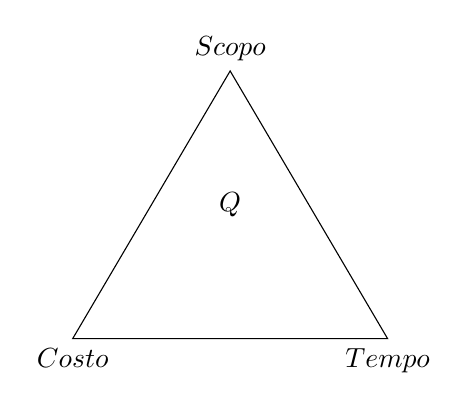
\begin{tikzpicture}
    \draw (0,0) node[anchor=north]{$Costo$}
        -- (4,0) node[anchor=north]{$Tempo$}
        -- (2,3.4) node[anchor=south]{$Scopo$}
        -- cycle    
        (2, 1.7) node[anchor=center]{$Q$};
\end{tikzpicture}
\caption{Triangolo dal triplice vincolo}
\label{t}
\end{figure}
Come è possibile visualizzare, nel caso in cui si dovesse dare più importanza ad uno di questi vincoli il triangolo non sarebbe più equilatero e bisognerebbe andare ad investire/magari perdere tempo per ri-aggiustarlo.
Molte volte è possibile trovare al centro una Q di Quality, questo fa riferimento ad una politica aziendale del cliente soddisfatto, \textit{\textcolor{red}{Total Quality Management}}, ossia si da la massima attenzione alla qualità del prodotto e ad offrire servizi ai clienti.

\section{Definizione di PMBOK e Project Management}
Nell'ultimo decennio si è visto come il concetto di progetto si sia diffuso sempre di più nelle varie aziende, e ciò ha portato alla necessità di metologie per gestirlo.
I motivi della sua diffusione sono tanti e ben distinti, ma possono essere riassunti in tre punti:
\begin{itemize}
    \item \textbf{Attività su commessa}
    \item \textbf{Problemi una tantum}
    \item \textbf{Strumento di innovazione}
\end{itemize}
La gestione del progetto attualemte è una vera e propria disciplina che prende il nome di \textbf{Project Management}.
Come concetti base della disciplina si può parlare di \textbf{CPM} (Critical Path Method, ossia di lavorare nella peggiore delle ipotesi per essere pronti ad ogni evenienza), il \textbf{PERT} (Program Evalutation and Review Tecnique, ossia valutare tempo e costo in rapporto ai rischi) ed il diagramma di \textbf{Gantt} (Utile per la gestione del tempo tramite piccole scadenze prefissate).
Tutto ciò viene descritto e ben spiegato nel \textbf{Project Management Body of Knowledge} che consiste in una vera e propria guida manageriale che ha lo scopo di definire linee guida per la gestione ed elaborazione di un progetto.

\subsection{Aree di Gestione}
Per descrivere le linee guida della gestione del progetto il PMBOK fa riferimento a 10 aree di gestione da membri diversi del gruppo.
\begin{enumerate}
    \item Gestione dell'ambito
    \item Gestione dei tempi
    \item Gestione dei costi
    \item Gestione della qualità
    \item Gestione delle risorse umane
    \item Gestione della comunicazione
    \item Gestione del rischio
    \item Gestione delle forniture
    \item Gestione delle integrazione dei processi
\end{enumerate}

\section{Figure del Project Management}

Le figure di un progetto e ciò che gli stessi devono fare/pensare può essere schematizzato con questo schema:

\begin{figure}

\begin{center}
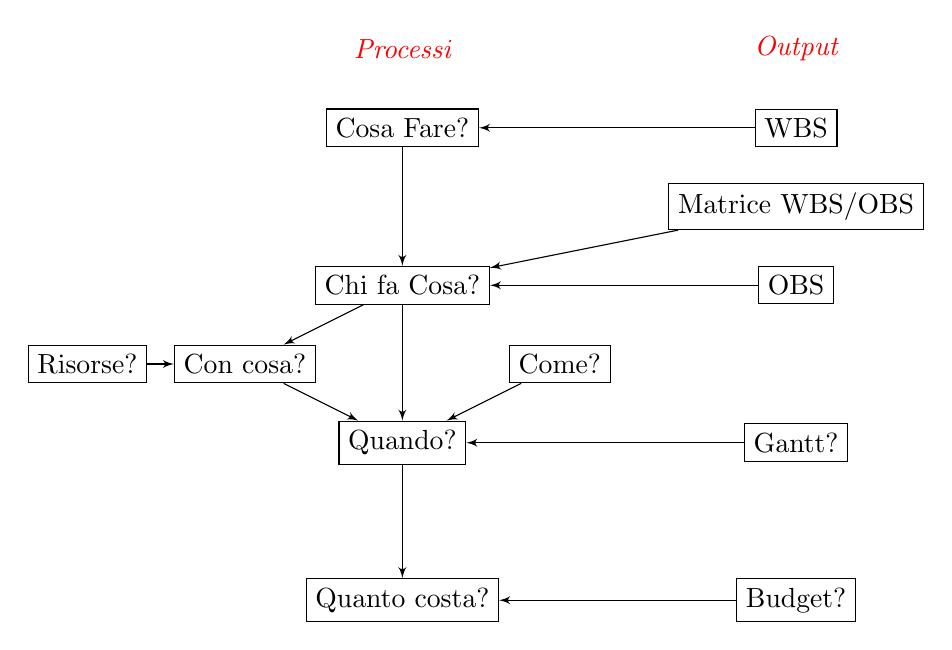
\begin{tikzpicture}
\node at (0, 1) {\textit{\textcolor{red}{Processi}}};
\node at (5, 1) {\textit{\textcolor{red}{Output}}};

\node[draw, rectangle] (s1) at (0,0) {Cosa Fare?};
\node[draw, rectangle] (t1) at (5,0) {WBS};

\node[draw,rectangle] (s2) at (0,-2) {Chi fa Cosa?};
\node[draw,rectangle] (t2) at (5,-2) {OBS};
\node[draw,rectangle] (t21) at (5,-1) {Matrice WBS/OBS};

\node[draw,rectangle] (s3) at (-2,-3) {Con cosa?};
\node[draw,rectangle] (t3) at (2,-3) {Come?};
\node[draw,rectangle] (t31) at (-4,-3) {Risorse?};


\node[draw,rectangle] (s4) at (0,-4) {Quando?};
\node[draw,rectangle] (t4) at (5,-4) {Gantt?};

\node[draw,rectangle] (s5) at (0,-6) {Quanto costa?};
\node[draw,rectangle] (t5) at (5,-6) {Budget?};
\path
    (t1) edge[->, >=latex', ] (s1)
    (s1) edge[->, >=latex', ] (s2)
    (t2) edge[->, >=latex', ] (s2)
    
    (s2) edge[->, >=latex', ] (s3)
    (s4) edge[->, >=latex']   (s5)
    (t31) edge[->, >=latex'] (s3)
    
    (t21) edge[->, >=latex',] (s2)
    (s3)  edge[->, >=latex'] (s4)
    (t3)  edge[->, >=latex'] (s4)
    (s2)  edge[->, >=latex'] (s4)
    (t4) edge[->, >=latex', ] (s4)
    (t5) edge[->, >=latex', ] (s5);
\end{tikzpicture}
\end{center}
\label{Schema}
\caption{Schema organizzativo}
\end{figure}

In una azienda, a gestire l'organizzazione e lo sviluppo di un progetto, è possibile trovare svariate figure che variano a seconda del tipo di azienda e progetto.
Una figura in comune per il Project Management è sicuramente quella del \textbf{Project Management}.
È la figura più importante, definito anche regista del progetto, lui non si preoccupa delle competenze tecniche ma di supervisione e coordinare tutti i membri del gruppo.
Si occupa di individuare la struttura di un progetto e di avviarla rispettando i vincoli (vedi Fig \ref{t}), deve organizzare un sistema di monitoraggio, una documentazione e cosa più importante prendere decisione sul \textbf{Make Or Buy}.

\chapter{Fasi Di un Progetto}
Un progetto nasce da una idea/opportunità per arrivare ad un risultato, ponendosi degli obiettivi.
Ogni obiettivo è raggiungibile mediante sforzi coordinati da parte del gruppo di lavoro seguendo delle fasi.
Generalmente le fasi si dividono in 4:

\begin{enumerate}
\item Concezione
\item Definizione
\item Realizzazione
\item Chiusura	
\end{enumerate}

Ciò avviene per ottimizzare al massimo la produttività ed limitare al massimo gli sprechi.
Vi sono nelle varie fasi(sopratutto nella prima) un ampio studio di tutti i vincoli e delle opportunità.
Il vincolo consiste in qualcosa che rende difficile la realizzazione del progetto.
Una oppurtunità è soluzione non prevista nel progetto che integrata possa aumentare la qualità dell'ultimo.
Volendo le varie fasi possono essere viste sottoforma di grafico cartesiano:
sulla ascissa troviamo il tempo t(mesi/anni, dipende dalla scadenza) e sulle ordinate il costo c(rappresentabile come un ritardo ed uno spreco di soldi).
Il grafico risultate è il seguente:
\begin{figure}[h!]
\begin{tikzpicture}
\begin{axis}[
    axis lines = left,
    xlabel = \(t\),
    ylabel = {\(c(t)\)},
    xmin=0, xmax=12,
    ymin=0, ymax=100000,
]
\addplot [
    color=red,
]
coordinates {
    (0,0)(2,0)(4,500)(6,1000)(8,3000)(10,10000)(12,100000)
    };
\addlegendentry{Bad Year}
\\
\addplot [
    color=blue,
]
coordinates {
    (0,0)(2,0)(4,500)(6,1000)(8,1500)(10,1700)(12,4000)
    };
\addlegendentry{Good Year}

\end{axis}
\end{tikzpicture}
\caption{Grafico andamento del Progetto}
\label{grap1}
\end{figure}

Come si può vedere la grafico, la linea rossa ha avuto grossi ritardi con un enorme spreco in termini di soldi: ciò è dovuto ad una brutta organizzazione iniziale.
Invece la linea blu è una sorta di condizione ideale nel caso in cui tutto fosse perfetto(avere dei ritardi e delle perdite durante la realizzazione del progetto è quasi normale, se ovviamente non eccessive)

\section{Concezione, analisi della fattibilità del progetto e tecniche di analisi}
La concezione di un progetto è la nascita dell'idea e la comprensione della sua fattibilità.
La concezione può essere divisa in sottoparti:

\subsection{Analisi Situazione Attuale}
Si descrive il contesto(\textcolor{blue}{dominio del software}) applicativo del progetto descrivendo le esigenze degli utenti sia interni che esterni.
Viene in oltre svolta l'\textbf{Analisi Situazione Attuale del Software}, vengono \textbf{Identificare i Vincoli di Origine Ambientale} quindi bisogna tenere conto di tutti i vincoli ambientali, normativi, temporali ed economici e chiedere consigli ad esperti del mestiere(notai, ambientalisti,investiri).
Si svolge una \textbf{Analisi della Realtà} in cui un vincolo diviene una opportunità, ossia si crea una situazione nuova e di successo.

Infine si \textbf{Definiscono gli obiettivi del progetto in termini quantitativi sintetici}:
Per definire gli obiettivi in maniera realistica e concreta, quindi senza andare in contro a perdite di tempo od uscire dai vincoli(vedi Fig \ref{t}) predisposti, ci sono delle tecniche come
la \textbf{\textcolor{blue}{S.M.A.R.T.}}:
\begin{itemize}
	\item \textbf{Specifici:} Deve essere dettagliato ed espresso chiaramente
	\item \textbf{Misurabili:} Quantificatore che indica la qualità (es. 10\% più grande...).
	\item \textbf{Accordati:} Deve essere concordato con tutti i membri del progetto.
	\item \textbf{Realistici:} Deve rispettare i vincoli del progetto (vedi Fig \ref{t}) e le 										capacità dei membri.
	\item \textbf{Temporalmente Definito:} Inserire una data di scandeza/consegna da rispettare.
\end{itemize}
Altra tecnica è la \textbf{\textcolor{blue}{S.W.O.T.}}, ossia Strenght, Weakness, Opportunities e Threat.
Questi punti costruscono una tabella che conterrà i vari punti di forza e debolezza sia dovuti a fattori interni(Strenght e Weakness) sia ad esterni(Opportunities e Threat):

\begin{table}[h!]
\begin{center}
\begin{tabular}{ |c|c|c|c| } 
 \hline
 S & W & O & T \\ [0.5ex] 
 \hline\hline
 cell1 & cell2 & cell3 & cell4 \\
 cell5 & cell6 & cell7 & cell8 \\
 \hline
\end{tabular}
\end{center}
\caption{Tabella S.W.O.T.}
\label{swot}
\end{table}




\subsection{Definizione di Massima del progetto:}
Essa si dividi in
\begin{itemize}
    \item \textbf{Definizione dei requisiti:} Sono le condizioni che il sistema deve rispettare. 		Compito del progettista elaboare una proposta di soluzione con lo scopo di
    \begin{enumerate}
        \item Identificare come deve fare il sistema informativo per rispondere alle esigenze della gente(\textbf{Requisiti funzionali}).
        \item Precisare i confini dell'applicazione e le modalità di iterazione con l'ambiente(\textbf{Requisiti di interfaccia}).
        \item .
        \item Definire l'elenco dei requisiti
        \item Elaborare le contradizione tra requisiti
        \item Identificare e mantenere il tracciamento tra requisiti utente e requisiti software.
    \end{enumerate}
    \item \textbf{Definire in linea di massima le specifiche del sistema:} architettura dei dati, architettura applicativa ed interfaccia utente.
    \item \textbf{Scelta delle modalità di realizzazione del progetto:} MakeOrBuy, riuso dei componenti esistenti, manutenzioni del sistema,formazione ed assistenza utente.
\end{itemize}


\subsection{Risk BreakDown Structure(RBS)}
Durante la stesura di un progetto il \textbf{rischio} è un evento/condizione che, nel caso dovesse succedere, avrebbe effetti negativi sul progetto stesso.
Sono presenti due fattori da tenere in considerazione: La \textbf{Probabilità} che il fenomeno avvenga e l' \textbf{Impatto} dello stesso, con le dovute conseguenze.
La gestione dei rischi è un processo di \textbf{Prevenzioni} in quanto bisogna evitare ogni possibile rischio, di \textbf{Mitigazione} ossia che bisogna adottare provvedimenti per la riduzione degli effetti indesiderati e di \textbf{Gestione delle conseguenze} predisporre in anticipo precauzioni nel caso il rischio avvenga e adottare provvedimenti per risolverlo.
Il RBS è una delle 10 aree di conoscenza del PMBOK, sono presenti 6 procedimenti che garantiscono la completa gestione dei rischi:
\begin{itemize}

 \item \textbf{Pianificazione della Gestione dei Rischi:} (Plan Risk Management)
 
 \item \textbf{Identificazione Dei Rischi}: (Identify Risk)
 
 \item \textbf{Analisi Quantitativa dei Rischi}:(Perform Qualitative Risk Analysis)
 
 \item \textbf{Analisi Quantitativa dei Rischi}:(Perform Quantitative Risk Analysis)
 
 \item \textbf{Pianificazione della Risposta ai Rischi}:(Plan Risk Responses)
 
 \item \textbf{Monitoraggio e Controllo Rischi}:(Control Risks)
\end{itemize}

Quindi il RBS serve proprio per evitare tutte le situazioni di \textbf{Crisis Managemnt}, ottimizzare i costi previsti con la dovuta gestione dei costi, aumentare le probabilità di successo e promuovere le oppurtunità.

In questa fase le attività del Project Manager sono due:
\begin{enumerate}

	\item \textbf{Individuare Fattori di Rischio}: Individuare delle aree in cui è possibile che arrivino dei rischi(punti deboli dell'azienda)
	\item \textbf{La Definizione}: Fornire una documentazione dei vari fattori di rischi, fornirne un livello quantitativo ed il motivo, come rappresentato nella tabella sottostante:
\begin{table}[h!]
\begin{center}
\begin{tabular}{ |c|c|c| } 
 	\hline
 	Fattori di rischio & Parametri & Livello \\ [0.5ex] 
 	\hline
 	Complessità gestionale & 
 	Organizzazion personale & 
 	\quantities{Ampia azienda\\Alto Rischio} \\
 				
 	\hline
 	Innovazione Tecnologica & 
 	\quantities{Utilizzo nuovo hardware,\\aggionrare apparecchiature} & 
 	\quantities{Apparecchiature recenti,\\personale esperto\\Basso rischio} \\
 				\hline
 				
\end{tabular}
\end{center}
\caption{Tabella dei Rischi}
\label{trischi}
\end{table}

Una volta stipulata la tabella di rischio si passa alla stesura della matrice di probabilità di impatto.
\begin{quote}
Date come variabili: \[F_r = probabilita'\]\[x_0 = impatto\] 
\end{quote}

Il nostro indice di probabilità \(F_r\) rappresenta la probabilità di avvenimento di un evento suddiviso in:
\begin{quote}
Bassa: \begin{math}P < 20\% \Longrightarrow F_r = 1\end{math}.\\
Media: \begin{math} 20 \leq P \leq 50\% \Longrightarrow F_r = 2\end{math}.\\
Alta: \begin{math}P < 50\% \Longrightarrow F_r = 3\end{math}.\\
\end{quote}

Il nostro indice d'impatto \(x_0\) viene calcolato in base al contesto:
\begin{quote}
Tempo: \begin{math} x_t = 1	\wedge x_t = 2 \wedge x_t = 3\end{math} influenza il tempo richiesto.\\
Costo: \begin{math} x_c = 1	\wedge x_c = 2 \wedge x_c = 3\end{math} incremento dei costi.\\
Prestazioni: \begin{math} x_p = 1	\wedge x_p = 2 \wedge x_p = 3\end{math} riduzione della qualità.	\\
\end{quote}



\end{enumerate}
\end{document}